\documentclass[a4paper, 12pt]{article}
\usepackage[utf8]{inputenc}
\usepackage[T1]{fontenc}
\usepackage[ngerman]{babel}
\usepackage{geometry}
\usepackage{listings}
\usepackage{xcolor}
\usepackage{hyperref}
\usepackage{helvet}
\usepackage{titlesec}
\usepackage{setspace}
\usepackage{graphicx}
\usepackage{pdfpages}
\usepackage{fancyhdr}
\usepackage{float}
\usepackage{enumitem}
\usepackage{tikz}
\usepackage{etoolbox}
\usepackage{tabularx}
\usepackage[style=apa, backend=biber, date=iso8601, urldate=iso8601]{biblatex}

%\addbibresource{bibs/citavi.bib}

%\DeclareFieldFormat{urldate}{
%    Abgerufen am \thefield{urlday}\adddot\addspace\mkbibmonth{\thefield{urlmonth}}\addspace\thefield{urlyear} von
%}

\hypersetup{breaklinks=true}

\definecolor{green}{HTML}{34A853}
\definecolor{orange}{HTML}{FBBC05}
\definecolor{red}{HTML}{EA4335}

\lstdefinelanguage{JavaScript}{
    keywords={break, case, catch, continue, debugger, default, delete, do, else, finally, for, function, if, in, instanceof, new, return, switch, this, throw, try, typeof, var, void, while, with},
    keywordstyle=\color{blue}\bfseries,
    ndkeywords={class, const, enum, export, extends, import, super, implements, interface, let, package, private, protected, public, static, yield, null, true, false},
    ndkeywordstyle=\color{darkgray}\bfseries,
    identifierstyle=\color{black},
    sensitive=false,
    comment=[l]{//},
    morecomment=[s]{/*}{*/},
    commentstyle=\color{purple}\ttfamily,
    stringstyle=\color{red}\ttfamily,
    morestring=[b]',
    morestring=[b]"
}

\lstset{
    language=JavaScript,
    extendedchars=true,
    basicstyle=\footnotesize\ttfamily,
    showstringspaces=false,
    showspaces=false,
    numbers=left,
    numberstyle=\footnotesize,
    numbersep=9pt,
    tabsize=2,
    breaklines=true,
    showtabs=false,
    captionpos=b
}
\geometry{a4paper, left=2.5cm, right=2.5cm, top=3cm, bottom=3cm, headsep=1.5cm}

\setlength{\parindent}{0pt}
\setlength{\parskip}{6pt}
\graphicspath{ {./images/} }

\pagestyle{fancy}
\fancyhf{}
\rhead{\vspace{0.2cm}
\includegraphics[width=4cm]{hs_mainz_logo}}
\fancypagestyle{plain}{
    \fancyhf{}
    \rhead{\vspace{0.2cm}
\includegraphics[width=4cm]{hs_mainz_logo}}
}
\renewcommand{\headrulewidth}{0pt}
\renewcommand{\footrulewidth}{0pt}
\fancyfoot[C]{\thepage}

\newcounter{lastroman}
\newrobustcmd{\switchtopage}[1]{
    \clearpage
    \setcounter{lastroman}{\value{page}}
    \pagenumbering{#1}
}
\newrobustcmd{\switchback}{
    \clearpage
    \pagenumbering{Roman}
    \setcounter{page}{\value{lastroman}}
}

% Document
\begin{document}

    \pagenumbering{Roman}

    \begin{titlepage}
    \centering
    \vspace*{1cm}

    
\includegraphics[width=0.4\textwidth]{hs_mainz_logo}\\
    \vspace{1.5cm}

    \textbf{\LARGE Praxismodul I}\\
    \vspace{0.5cm}
    \textbf{\Large Collectiqo}\\
    \vspace{1.5cm}

    \textbf{Hochschule Mainz}\\
    \vspace{0.5cm}
    Fachbereich Wirtschaft\\
    \vspace{0.5cm}
    B.Sc. Wirtschaftsinformatik dual\\
    \vspace{1.5cm}

    \textbf{Authors:}\\
    Bindernagel, Lorenz\\
    Schäfer, Robin\\
    Šimić, Darko\\
    Struve, Anika\\
    \vfill

    \today
\end{titlepage}
    \newpage

    \textbf{Nützliche Informationen:}\par
\vspace{0.5cm}
GitHub Repository: \url{https://github.com/LorackDev/collectiqo}\par
Datei für die Umgebungsvariablen ist nicht im Repository hinterlegt!\par
\vspace{0.5cm}
Dockerhub Hauptapplikation: \url{https://hub.docker.com/repository/docker/lorackdev/clq-app/general}\par
Dockerhub Custom MySQL: \url{https://hub.docker.com/repository/docker/lorackdev/clq-mysql/general}\par
Dockerhub Custom MongoDB: \url{https://hub.docker.com/repository/docker/lorackdev/clq-mongodb/general}\par
    \newpage

    \setcounter{page}{2}
    \tableofcontents
    \newpage

    \switchtopage{arabic}

    \section{Projektplanung- und Management}\label{sec:section-one}

Lorenz ipsum dolor sit amet, consetetur sadipscing elitr, sed diam nonumy eirmod tempor invidunt ut labore et dolore magna aliquyam erat, sed diam voluptua.
At vero eos et accusam et justo duo dolores et ea rebum.
Stet clita kasd gubergren, no sea takimata sanctus est Lorem ipsum dolor sit amet.
Lorenz ipsum dolor sit amet, consetetur sadipscing elitr, sed diam nonumy eirmod tempor invidunt ut labore et dolore magna aliquyam erat, sed diam voluptua.
At vero eos et accusam et justo duo dolores et ea rebum.
Stet clita kasd gubergren, no sea takimata sanctus est Lorem ipsum dolor sit amet.

\subsection{Rückblick auf Praxismodul I}\label{subsec:subsection-one-one}

Lorenz ipsum dolor sit amet, consetetur sadipscing elitr, sed diam nonumy eirmod tempor invidunt ut labore et dolore magna aliquyam erat, sed diam voluptua.
At vero eos et accusam et justo duo dolores et ea rebum.
Stet clita kasd gubergren, no sea takimata sanctus est Lorem ipsum dolor sit amet.
Lorenz ipsum dolor sit amet, consetetur sadipscing elitr, sed diam nonumy eirmod tempor invidunt ut labore et dolore magna aliquyam erat, sed diam voluptua.
At vero eos et accusam et justo duo dolores et ea rebum.
Stet clita kasd gubergren, no sea takimata sanctus est Lorem ipsum dolor sit amet.

\subsection{Zielsetzungen im Praxismodul II}\label{subsec:subsection-one-two}

Lorenz ipsum dolor sit amet, consetetur sadipscing elitr, sed diam nonumy eirmod tempor invidunt ut labore et dolore magna aliquyam erat, sed diam voluptua.
At vero eos et accusam et justo duo dolores et ea rebum.
Stet clita kasd gubergren, no sea takimata sanctus est Lorem ipsum dolor sit amet.
Lorenz ipsum dolor sit amet, consetetur sadipscing elitr, sed diam nonumy eirmod tempor invidunt ut labore et dolore magna aliquyam erat, sed diam voluptua.
At vero eos et accusam et justo duo dolores et ea rebum.
Stet clita kasd gubergren, no sea takimata sanctus est Lorem ipsum dolor sit amet.

\subsection{Projektorganisationen}\label{subsec:subsection-one-three}

Lorenz ipsum dolor sit amet, consetetur sadipscing elitr, sed diam nonumy eirmod tempor invidunt ut labore et dolore magna aliquyam erat, sed diam voluptua.
At vero eos et accusam et justo duo dolores et ea rebum.
Stet clita kasd gubergren, no sea takimata sanctus est Lorem ipsum dolor sit amet.
Lorenz ipsum dolor sit amet, consetetur sadipscing elitr, sed diam nonumy eirmod tempor invidunt ut labore et dolore magna aliquyam erat, sed diam voluptua.
At vero eos et accusam et justo duo dolores et ea rebum.
Stet clita kasd gubergren, no sea takimata sanctus est Lorem ipsum dolor sit amet.

\subsection{Tools}\label{subsec:subsection-one-four}

Lorenz ipsum dolor sit amet, consetetur sadipscing elitr, sed diam nonumy eirmod tempor invidunt ut labore et dolore magna aliquyam erat, sed diam voluptua.
At vero eos et accusam et justo duo dolores et ea rebum.
Stet clita kasd gubergren, no sea takimata sanctus est Lorem ipsum dolor sit amet.
Lorenz ipsum dolor sit amet, consetetur sadipscing elitr, sed diam nonumy eirmod tempor invidunt ut labore et dolore magna aliquyam erat, sed diam voluptua.
At vero eos et accusam et justo duo dolores et ea rebum.
Stet clita kasd gubergren, no sea takimata sanctus est Lorem ipsum dolor sit amet.
    \newpage
    
    \section{Überarbeitung und Erweiterung des New Collection Modals}\label{sec:uberarbeitung-und-erweiterung-des-new-collection-modals}

Das New Collection Modal ist die zentrale Schnittstelle zur Erstellung einer neuen Sammlung auf der Collectiqo-Plattform.
Es ermöglicht Nutzer:innen, grundlegende Eigenschaften wie Presets, Farbauswahl, Name und optional benutzerdefinierte Felder festzulegen.
Im aktuellen Praxismodul wurde das Modal sowohl funktional als auch visuell überarbeitet.

%
\subsection{Frontend}\label{subsec:new-collection-frontend}

Die visuelle und funktionale Überarbeitung des Collection-Modals im aktuellen Praxismodul stellt eine wesentliche Erweiterung gegenüber der vorherigen Version dar.
Abbildung \ref{fig:modal-old} zeigt das ursprüngliche Modal aus dem vorangegangenen Semester.
Hier war es lediglich möglich, eine neue Sammlung durch Auswahl eines vordefinierten Presets zu erstellen.
Benutzerdefinierte Felder konnten nicht ergänzt werden, ebenso fehlte die Möglichkeit, Farben oder Bilder zu hinterlegen.
Für die benutzerdefinierten Felder sowie die Farbauswahl existierten zwar bereits die Frontend Buttons, jedoch waren diese nicht funktional bzw. das Backend konnte mit der Auswahl noch nicht umgehen.

\begin{figure}[H]
    \centering
    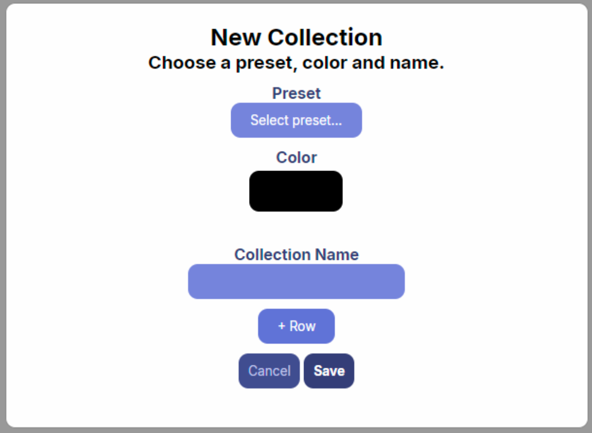
\includegraphics[width=0.6\textwidth]{modal_old}
    \caption{Ursprüngliches Collection-Modal (Praxismodul II)}
    \label{fig:modal-old}
\end{figure}

Die überarbeitete Version, dargestellt in Abbildung~\ref{fig:modal-new}, erweitert diesen Funktionsumfang deutlich.
Neben einer visuell zentrierten und optisch konsistenten Gestaltung wurden mehrere neue Eingabemöglichkeiten ergänzt: Nutzer können nun eigene Felder definieren sowie ein Bild hochladen.
Diese Funktionen korrespondieren direkt mit der im Abschnitt \ref{subsubsec:save-new-collection} beschriebenen Speicherung im Backend.

\begin{figure}[H]
    \centering
    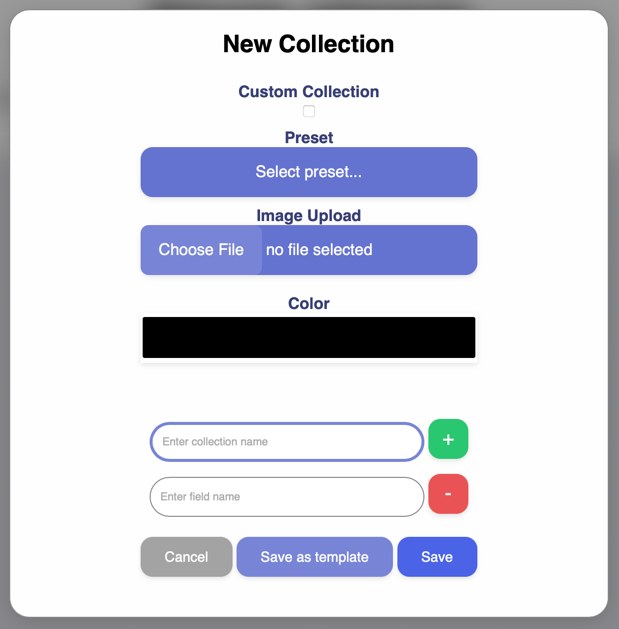
\includegraphics[width=0.6\textwidth]{modal_new}
    \caption{Überarbeitetes Collection-Modal (Praxismodul III)}
    \label{fig:modal-new}
\end{figure}

Zusätzlich zu diesen Eingabefeldern wurden zwei Schaltflächen implementiert: „Save“ und „Save as template“.
Über „Save“ wird die Sammlung wie in Abschnitt \ref{subsubsec:save-new-collection} beschrieben direkt gespeichert, während „Save as template“ eine Vorlage erstellt, die beim nächsten Öffnen des Modals im Preset-Menü ausgewählt werden kann (siehe Abschnitt \ref{subsubsec:save-as-template}).
Beim Wechsel eines Presets wird das Modal dynamisch mit den entsprechenden Daten befüllt – diese Funktionalität ist ebenfalls im Backend dokumentiert (vgl. Abschnitt \ref{subsubsec:load-template-data}).

\subsection{Backend}\label{subsec:new-collection-backend}

Parallel zur Überarbeitung des Frontends wurde auch das Backend des New Collection Modals grundlegend erweitert.
Während im vorherigen Semester lediglich das Erstellen einer Sammlung anhand vordefinierter Presets möglich war, unterstützt das System nun eine deutlich flexiblere und funktionsreichere Erstellung.

\subsubsection{Speichern einer individuellen Sammlung}\label{subsubsec:save-new-collection}

Beim Klick auf den „Save“-Button werden alle eingegebenen Daten – der Sammlungsname, die benutzerdefinierten Spaltennamen, ein Bild sowie eine gewählte Farbe – über ein \texttt{FormData}-Objekt an den Endpunkt \texttt{/create-new-collection} gesendet:

\begin{lstlisting}[language=JavaScript, caption=Clientseitiges Speichern einer neuen Sammlung]
const formData = new FormData();
formData.append('name', collectionName);
formData.append('columns', JSON.stringify(columns));
formData.append('color', color);
formData.append('imageUpload', file);

const response = await fetch('/create-new-collection', {
    method: 'POST',
    body: formData
});
\end{lstlisting}

Der Server verarbeitet diese Daten und speichert die Inhalte in der Datenbank.
Das Bild wird in der MongoDB als Binärdaten abgelegt, die Farbe als Textwert gespeichert.
Die so gespeicherte Sammlung erscheint anschließend in der Übersicht.
Leider wird im Frontend die Auswahl der Farbe und des Bilds nicht weiter verwertet.

Der API-Endpunkt \texttt{/create-new-collection} wird durch den \texttt{createNewCollectionController} verarbeitet, der intern den \texttt{createNewCollectionService} aufruft.
Dieser wurde im aktuellen Praxismodul dahingehend erweitert, dass neben dem Namen, den Spalten und dem Benutzername nun auch ein Bild (als Binärdaten) sowie ein Farbwähler-Wert verarbeitet und in der Datenbank gespeichert werden können.

\begin{lstlisting}[language=JavaScript, caption=Service-Aufruf im Controller]
await createNewCollectionService(
    name,
    parsedColumns,
    username,
    imageBuffer,
    imageType,
    color
);
\end{lstlisting}

Die Speicherung erfolgt in der MongoDB-Collection \texttt{collections} über folgenden Datenbankeintrag:

\begin{lstlisting}[language=JavaScript, caption=Dokumentstruktur im Service]
const doc = {
    name: name,
    columns: columns,
    username: username,
    entries: [],
    color: color,
    image: imageBuffer,
    imageType: imageType
};

const result = await collection.insertOne(doc);
\end{lstlisting}

\subsubsection{Speichern einer Sammlung als Template}\label{subsubsec:save-as-template}

Alternativ zum direkten Speichern kann eine Sammlung auch als Vorlage hinterlegt werden.
Dies geschieht über den „Save as template“-Button, der die Daten an den Endpunkt \texttt{/create-template} sendet:

\begin{lstlisting}[language=JavaScript, caption=Clientseitiges Speichern einer Sammlung als Vorlage]
const formData = new FormData();
formData.append('name', templateName);
formData.append('columns', JSON.stringify(columns));
formData.append('color', color);

const file = document.getElementById('imageUpload').files[0];
if (file) {
    formData.append('imageUpload', file);
}

await fetch('/create-template', {
    method: 'POST',
    body: formData
});
\end{lstlisting}

Der API-Endpunkt \texttt{/create-template} wird durch den \texttt{createTemplateController} verarbeitet.
Dieser ruft intern den \texttt{createTemplateService} auf und übergibt die extrahierten Daten des Formulars, einschließlich der optionalen Bild- und Farbangaben:

\begin{lstlisting}[language=JavaScript, caption=Service-Aufruf im Controller]
await createTemplateService({
    ...templateData,
    image: templateData.imageBuffer,
    imageType: templateData.imageType
});
\end{lstlisting}

Im Service erfolgt die Speicherung des Templates in der Collection \texttt{templates} der Datenbank \texttt{clq\_collections}.
Die Methode wurde im aktuellen Praxismodul erweitert, um Bilddaten als Buffer sowie den MIME-Type zu verarbeiten und dauerhaft zu speichern:

\begin{lstlisting}[language=JavaScript, caption=Speicherung im createTemplateService]
const templatesCollection = db.collection('templates');

await templatesCollection.insertOne({
    ...templateData,
    image: templateData.imageBuffer,
    imageType: templateData.imageType
});
\end{lstlisting}

Durch diese Erweiterung ist es nun möglich, Vorlagen nicht nur mit strukturellen Informationen (z.B. Spaltennamen), sondern auch mit visuellen Eigenschaften wie Farbe und Bild zu versehen.
Diese Templates stehen beim nächsten Öffnen des Modals im Preset-Auswahlfeld zur Verfügung.
Das System lädt die verfügbaren Templates beim Initialisieren des Modals über eine GET-Anfrage:

\begin{lstlisting}[language=JavaScript, caption=Presets beim Laden des Modals laden]
fetch('/get-user-templates')
    .then(response => response.json())
    .then(templateNames => {
        const $presetSelect = document.getElementById('preset');
        $presetSelect.innerHTML = '<option value="x" disabled selected>Select preset...</option>';
        templateNames.forEach(name => {
            const option = document.createElement('option');
            option.value = name;
            option.textContent = name;
            $presetSelect.appendChild(option);
        });
    });
\end{lstlisting}

Der GET-Endpunkt \texttt{/get-user-templates} wird durch einen zugehörigen Controller verarbeitet, der intern den Service \texttt{getUserTemplatesServices(username)} aufruft.
Dieser Service liest alle Vorlagen aus der Collection \texttt{templates}, die entweder dem aktuellen Benutzer oder als global markiert (\texttt{owner: 'GLOBAL'}) gespeichert wurden.

\begin{lstlisting}[language=JavaScript, caption=Service zum Abrufen von Template-Namen]
const db = await connectToDb();
const templatesCollection = db.collection('templates');

const templates = await templatesCollection
    .find({ $or: [ { owner: username }, { owner: 'GLOBAL' } ] })
    .project({ name: 1 })
    .toArray();

return templates.map(template => template.name);
\end{lstlisting}

Dieser Service liefert ein Array von Namen zurück, das anschließend im Frontend in der Preset-Auswahl angezeigt wird.

\subsubsection{Dynamisches Befüllen durch Preset-Auswahl}\label{subsubsec:load-template-data}

Wird eine gespeicherte Vorlage ausgewählt, sendet das Frontend eine Anfrage, um die zugehörigen Felder, die gespeicherte Farbe und ggf. das Bild zu laden.
Anschließend werden die Eingabefelder entsprechend befüllt:

\begin{lstlisting}[language=JavaScript, caption=Preset-Auswahl lädt Felder und Bild]
const response = await fetch(`/get-preset-data?templateName=${selectedPreset}`);
const templateData = await response.json();

clearExistingFields();
populateFieldsFromTemplate(templateData);
setColorPickerValue(templateData.color);
\end{lstlisting}

\textbf{Backend-Logik:} Der GET-Endpunkt \texttt{/get-preset-data} ruft im Hintergrund den \texttt{getPresetDataService(preset)} auf.
Dieser Service wurde erweitert, um ein vollständiges Template-Objekt mit allen gespeicherten Werten zurückzugeben – einschließlich der dynamisch definierten Felder, der ausgewählten Farbe sowie optional des hinterlegten Bilds und dessen MIME-Type.

\begin{lstlisting}[language=JavaScript, caption=Service zum Laden eines Templates]
const getPresetDataService = async(preset) => {
let db;
try {
db = await connectToDb();
const templatesCollection = db.collection('templates');
if (typeof preset !== 'string') {
throw new Error('Invalid preset value');
}
        const template = await templatesCollection.findOne({ name: { $eq: preset } });

        if (template) {
            return template;
        } else {
            console.warn('No template found for preset:', preset);
            return {};
        }
    } catch (error) {
        console.error('Error fetching preset data:', error);
        return {};
    } finally {
        if (db) {
            await closeConnection();
        }
    }
}
\end{lstlisting}

Diese Funktion prüft zunächst die Gültigkeit des übergebenen Werts \texttt{preset}, stellt dann eine Verbindung zur Datenbank her und sucht in der Collection \texttt{templates} nach einem entsprechenden Eintrag.
Wird dieser gefunden, gibt der Service das gesamte Template-Objekt zurück.
Damit können im Frontend alle notwendigen Eingabefelder und Darstellungen korrekt initialisiert werden.

\subsubsection{Unterschied zum vorherigen Semester}\label{subsubsec:comparison-previous}

Im vorherigen Semester war ausschließlich das Erstellen von Sammlungen basierend auf fest programmierten Presets möglich.
Es bestand keine Möglichkeit, benutzerdefinierte Felder zu speichern oder die Sammlung visuell mit Farbe oder Bild anzureichern.
Die neuen Funktionen stellen daher einen erheblichen Fortschritt dar: Sie ermöglichen nicht nur eine flexible Sammlungserstellung, sondern erlauben es auch, Vorlagen für wiederkehrende Strukturen anzulegen und weiterzuverwenden.
    \newpage

    \section{zAnika}\label{subsec:zAnika}

Lorenz ipsum dolor sit amet, consetetur sadipscing elitr, sed diam nonumy eirmod tempor invidunt ut labore et dolore magna aliquyam erat, sed diam voluptua.
At vero eos et accusam et justo duo dolores et ea rebum.
Stet clita kasd gubergren, no sea takimata sanctus est Lorenz ipsum dolor sit amet.

\subsection{SubthemaAnika1}\label{subsubsec:anika1}

Lorenz ipsum dolor sit amet, consetetur sadipscing elitr, sed diam nonumy eirmod tempor invidunt ut labore et dolore magna aliquyam erat, sed diam voluptua.
At vero eos et accusam et justo duo dolores et ea rebum.
Stet clita kasd gubergren, no sea takimata sanctus est Lorenz ipsum dolor sit amet.

\subsection{SubthemaAnika2}\label{subsubsec:anika2}

Lorenz ipsum dolor sit amet, consetetur sadipscing elitr, sed diam nonumy eirmod tempor invidunt ut labore et dolore magna aliquyam erat, sed diam voluptua.
At vero eos et accusam et justo duo dolores et ea rebum.
Stet clita kasd gubergren, no sea takimata sanctus est Lorenz ipsum dolor sit amet.

\subsection{SubthemaAnika3}\label{subsubsec:anika3}

Lorenz ipsum dolor sit amet, consetetur sadipscing elitr, sed diam nonumy eirmod tempor invidunt ut labore et dolore magna aliquyam erat, sed diam voluptua.
At vero eos et accusam et justo duo dolores et ea rebum.
Stet clita kasd gubergren, no sea takimata sanctus est Lorenz ipsum dolor sit amet.


    \newpage

    \section{zDarko}\label{subsec:zDarko}

Lorenz ipsum dolor sit amet, consetetur sadipscing elitr, sed diam nonumy eirmod tempor invidunt ut labore et dolore magna aliquyam erat, sed diam voluptua.
At vero eos et accusam et justo duo dolores et ea rebum.
Stet clita kasd gubergren, no sea takimata sanctus est Lorenz ipsum dolor sit amet.

\subsection{SubthemaDarko1}\label{subsubsec:darko1}

Lorenz ipsum dolor sit amet, consetetur sadipscing elitr, sed diam nonumy eirmod tempor invidunt ut labore et dolore magna aliquyam erat, sed diam voluptua.
At vero eos et accusam et justo duo dolores et ea rebum.
Stet clita kasd gubergren, no sea takimata sanctus est Lorenz ipsum dolor sit amet.

\subsection{SubthemaDarko2}\label{subsubsec:darko2}

Lorenz ipsum dolor sit amet, consetetur sadipscing elitr, sed diam nonumy eirmod tempor invidunt ut labore et dolore magna aliquyam erat, sed diam voluptua.
At vero eos et accusam et justo duo dolores et ea rebum.
Stet clita kasd gubergren, no sea takimata sanctus est Lorenz ipsum dolor sit amet.

\subsection{SubthemaDarko3}\label{subsubsec:darko3}

Lorenz ipsum dolor sit amet, consetetur sadipscing elitr, sed diam nonumy eirmod tempor invidunt ut labore et dolore magna aliquyam erat, sed diam voluptua.
At vero eos et accusam et justo duo dolores et ea rebum.
Stet clita kasd gubergren, no sea takimata sanctus est Lorenz ipsum dolor sit amet.


    \newpage

    \section{zLorenz}\label{subsec:zLorenz}

Lorenz ipsum dolor sit amet, consetetur sadipscing elitr, sed diam nonumy eirmod tempor invidunt ut labore et dolore magna aliquyam erat, sed diam voluptua.
At vero eos et accusam et justo duo dolores et ea rebum.
Stet clita kasd gubergren, no sea takimata sanctus est Lorenz ipsum dolor sit amet.

\subsection{}\label{subsubsec:lorenz1}

Lorenz ipsum dolor sit amet, consetetur sadipscing elitr, sed diam nonumy eirmod tempor invidunt ut labore et dolore magna aliquyam erat, sed diam voluptua.
At vero eos et accusam et justo duo dolores et ea rebum.
Stet clita kasd gubergren, no sea takimata sanctus est Lorenz ipsum dolor sit amet.

\subsection{SubthemaLorenz2}\label{subsubsec:lorenz2}

Lorenz ipsum dolor sit amet, consetetur sadipscing elitr, sed diam nonumy eirmod tempor invidunt ut labore et dolore magna aliquyam erat, sed diam voluptua.
At vero eos et accusam et justo duo dolores et ea rebum.
Stet clita kasd gubergren, no sea takimata sanctus est Lorenz ipsum dolor sit amet.

\subsection{SubthemaLorenz3}\label{subsubsec:lorenz3}

Lorenz ipsum dolor sit amet, consetetur sadipscing elitr, sed diam nonumy eirmod tempor invidunt ut labore et dolore magna aliquyam erat, sed diam voluptua.
At vero eos et accusam et justo duo dolores et ea rebum.
Stet clita kasd gubergren, no sea takimata sanctus est Lorenz ipsum dolor sit amet.


\subsection{Backend der Nutzereinstellungen}\label{subsec:backend-user-settings}

Im Rahmen des dritten Praxismoduls wurden mehrere Backend-Funktionalitäten für die Nutzereinstellungen implementiert.
Ziel war es, den Nutzern eine komfortable Möglichkeit zu bieten, ihre Kontoinformationen selbstständig zu verwalten.
Es wurden vier zentrale Funktionen umgesetzt: die Änderung des Benutzernamens, des Passworts, der E-Mail-Adresse sowie ein Logout-Service.
Diese Auswahl wurde mit dem Hintergrund der Zielsetzung für dieses Semester getroffen.
Für alle diese Funktionen existierte bereits eine Frontend implementierung, nun sollte auch das Backend eingebaut werden.
Die Implementierungen nutzt die etablierte MySQL für Benutzerdaten sowie MongoDB für sammlungsrelevante Daten.
Strukturell nutzen alle Funktionen die im Praxismodul II eingeführte Aufteilung in Route, Controller und Service.

\subsubsection{Ändern des Benutzernamens}\label{subsubsec:username-update}

Die Funktion zur Änderung des Benutzernamens prüft zunächst, ob der alte Benutzername existiert und ob der neue Benutzername bereits vergeben ist.
Anschließend wird der Name sowohl in der MySQL-Datenbank als auch in den relevanten MongoDB-Collections aktualisiert:

\begin{lstlisting}[language=JavaScript, caption=Überprüfung und Update des Usernamens in MySQL]
const results = await queryDatabase('SELECT * FROM clq_users WHERE username = ?', [oldUsername]);
const user = handleResults(results);

if (!user) {
    throw new Error('User not found');
}

const results = await queryDatabase('SELECT * FROM clq_users WHERE username = ?', [newUsername]);
if (handleResults(results)) {
    throw new Error('Username already in use');
}

await queryDatabase('UPDATE clq_users SET username = ? WHERE username = ?', [newUsername, oldUsername]);
\end{lstlisting}

Zusätzlich wird der Benutzername in MongoDB aktualisiert, um Konsistenz über alle Datenbanken hinweg sicherzustellen.

\subsubsection{Ändern des Passworts}\label{subsubsec:password-update}

Zur Änderung des Passworts wird zunächst das bisherige Passwort mittels `bcrypt.compare` validiert.
Anschließend wird das neue Passwort gehasht und in der Datenbank gespeichert:

\begin{lstlisting}[language=JavaScript, caption=Passwortvalidierung und Update]
const passwordMatches = await bcrypt.compare(oldPassword, user.password);
if (!passwordMatches) {
    throw new Error('Incorrect old password');
}

const hashedNewPassword = await bcrypt.hash(newPassword, 10);
await queryDatabase('UPDATE clq_users SET password = ? WHERE username = ?', [hashedNewPassword, username]);
\end{lstlisting}

Diese Sicherheitsmaßnahmen stellen sicher, dass nur authentifizierte Nutzer ihr Passwort ändern können.

\subsubsection{Ändern der E-Mail-Adresse}\label{subsubsec:email-update}

Die Änderung der E-Mail-Adresse erfolgt durch eine einfache Aktualisierung des entsprechenden Feldes in der MySQL-Datenbank.
Vorab wird überprüft, ob der Benutzername existiert:

\begin{lstlisting}[language=JavaScript, caption=Update der E-Mail-Adresse]
const results = await queryDatabase('SELECT * FROM clq_users WHERE username = ?', [username]);
const user = handleResults(results);

if (!user) {
    throw new Error('User not found');
}

await queryDatabase('UPDATE clq_users SET email = ? WHERE username = ?', [newEmail, username]);
\end{lstlisting}

\subsubsection{Logout-Funktionalität}\label{subsubsec:logout}

Der Logout-Prozess basiert auf der Zerstörung der Session des Nutzers.
Dies wurde durch die `req.session.destroy()` Methode realisiert.
Bei erfolgreicher Durchführung wird die Session beendet, andernfalls ein Fehler zurückgegeben:

\begin{lstlisting}[language=JavaScript, caption=Logout-Service über Session-Zerstörung]
req.session.destroy(err => {
    if (err) {
        return reject(new Error('Failed to logout'));
    }
    resolve();
});
\end{lstlisting}
    \newpage

    \section{vServer}\label{subsec:vserver}

Lorenz ipsum dolor sit amet, consetetur sadipscing elitr, sed diam nonumy eirmod tempor invidunt ut labore et dolore magna aliquyam erat, sed diam voluptua.
At vero eos et accusam et justo duo dolores et ea rebum.
Stet clita kasd gubergren, no sea takimata sanctus est Lorenz ipsum dolor sit amet.

\subsection{Hosting}\label{subsubsec:hosting}

Lorenz ipsum dolor sit amet, consetetur sadipscing elitr, sed diam nonumy eirmod tempor invidunt ut labore et dolore magna aliquyam erat, sed diam voluptua.
At vero eos et accusam et justo duo dolores et ea rebum.
Stet clita kasd gubergren, no sea takimata sanctus est Lorenz ipsum dolor sit amet.

\subsection{Automatisierung Updates}\label{subsubsec:automatisierung-updates}

Lorenz ipsum dolor sit amet, consetetur sadipscing elitr, sed diam nonumy eirmod tempor invidunt ut labore et dolore magna aliquyam erat, sed diam voluptua.
At vero eos et accusam et justo duo dolores et ea rebum.
Stet clita kasd gubergren, no sea takimata sanctus est Lorenz ipsum dolor sit amet.

\subsection{Reverse Proxy}\label{subsubsec:reverse-proxy}

Lorenz ipsum dolor sit amet, consetetur sadipscing elitr, sed diam nonumy eirmod tempor invidunt ut labore et dolore magna aliquyam erat, sed diam voluptua.
At vero eos et accusam et justo duo dolores et ea rebum.
Stet clita kasd gubergren, no sea takimata sanctus est Lorenz ipsum dolor sit amet.

Die Konfiguration des Nginx-Revers-Proxys erfolgte in der Datei \textit{nginx/nginx.conf} und sieht wie folgt aus:
\vspace{1em}
\begin{lstlisting}[label={lst:lst-nginx-config}]
events {
    worker_connections  1024;
}

http {
    server_tokens off;
    charset utf-8;
    server {
        listen 80 default_server;
        server_name collectiqo.de www.collectiqo.de collectiqo.com www.collectiqo.com;

        location ~ /.well-known/acme-challenge/ {
            root /var/www/certbot;
        }

        location / {
            return 301 https://collectiqo.com$request_uri;
        }
    }
    server {
        listen 443 ssl;
        server_name collectiqo.de www.collectiqo.de collectiqo.com www.collectiqo.com;

        ssl_certificate /etc/letsencrypt/live/collectiqo.com/fullchain.pem;
        ssl_certificate_key /etc/letsencrypt/live/collectiqo.com/privkey.pem;

        location ~ /.well-known/acme-challenge/ {
            root /var/www/certbot;
        }
        location / {
            #proxy_pass http://test-webserver;
            proxy_pass https://collectiqo-web-1:3000;
            proxy_http_version 1.1;
            proxy_set_header Host $host;
            proxy_set_header Upgrade $http_upgrade;
            proxy_set_header Connection 'upgrade';
            proxy_set_header X-Real-IP $remote_addr;
            proxy_set_header X-Forwarded-For $proxy_add_x_forwarded_for;
            proxy_set_header X-Forwarded-Proto $scheme;
            proxy_cache_bypass $http_upgrade;
        }
    }
}
\end{lstlisting}
\vspace{1em}

    \newpage

    \section{Fazit und Ausblick}\label{sec:fazit-ausblick}

Dieses Kapitel fasst die wichtigsten Erkenntnisse zusammen, beleuchtet Abweichungen von den ursprünglichen Zielen und reflektiert die Fortschritte des Projekts.
Gleichzeitig wird ein Ausblick auf zukünftige Schritte gegeben, um das Projekt weiterzuentwickeln und an neue Herausforderungen anzupassen.

\subsection{Abweichungen der geplanten Ziele}\label{subsec:abweichungen-der-geplanten-ziele}

Im Rahmen des Projekts konnten einige der gesetzten Ziele erfolgreich umgesetzt werden, während andere aufgrund unvorhergesehener Herausforderungen nicht erreicht wurden.

\begin{itemize}[noitemsep]
    \item \textbf{Restrukturierung der GitHub-Struktur}: Dieses Ziel wurde vollständig erreicht, wodurch eine klarere Organisation und Nachvollziehbarkeit des Projekts gewährleistet ist.
    \item \textbf{Auslagerung von redundanten Code-Snippets in HTML, CSS und JavaScript}: Die Reduktion von Redundanzen wurde erfolgreich umgesetzt, was die Wartbarkeit und Skalierbarkeit des Projekts deutlich verbessert hat.
    \item \textbf{Designanpassung mit richtigem Branding}: Das Branding wurde erfolgreich implementiert, was zu einem professionelleren und kohärenten Auftritt beiträgt.
    \item \textbf{Projektmanagement-Tool}: Der Wechsel auf ein neues Projektmanagement-Tool konnte zu Beginn des Praxismoduls II erfolgreich umgesetzt werden, was die Organisation und Kommunikation im Team verbessert hat.
    \item \textbf{Docker-Erweiterung}: Die Docker-Umgebung konnte erfolgreich um zwei Container (Reverse Proxy und Certbot Zertifikatsverwaltung) erweitert werden.
    \item \textbf{Bugs im Front- und Backend}: Die Behebung von Bugs wurde erfolgreich durchgeführt, was die Stabilität und Zuverlässigkeit der Plattform erhöht hat.
    \item \textbf{vServer-Hosting}: Die Plattform konnte erfolgreich auf einem vServer gehostet werden, was die Verfügbarkeit verbessert und die Grundlage für zukünftige Erweiterungen schafft.
    \item \textbf{DB-Constrains}: Die Absicherung der Datenbank durch Constraints konnte aus Zeitgründen nicht umgesetzt werden, bleibt aber ein Ziel für zukünftige Entwicklungen.
    \item \textbf{Integrationstests}: Die Implementierung von Integrationstests konnte ebenfalls nicht umgesetzt werden und verbleibt im Backlog.
    \item \textbf{Erweiterung der Funktionen für die Anpassung von Collections}: Dieses Ziel konnte nicht erreicht werden, da die notwendigen Umstrukturierungen und die Vereinheitlichung anderer Komponenten mehr Zeit in Anspruch nahmen als ursprünglich geplant.
\end{itemize}

\newpage

\subsection{Retrospektive}\label{subsec:retrospektive}

Im Vergleich zum ersten Semester haben wir uns bewusst weniger vorgenommen, um einen klaren Fokus auf die grundlegende Restrukturierung des Projektes zu legen.
Unser Hauptziel war es, die Wiederverwendbarkeit von Code zu ermöglichen und damit eine nachhaltige Grundlage für zukünftige Entwicklungen zu schaffen.
Die Teammitglieder konnten zudem gezielter persönlichen Interessen nachgehen und sich in spezifischen Bereichen vertiefen.

Ein weiterer Schwerpunkt lag auf der Verbesserung der Benutzerfreundlichkeit und der Gestaltung ansprechender Designs.
Diese Maßnahmen sollten sicherstellen, dass spätere Funktionserweiterungen ohne größere Rückschritte oder grundlegende Änderungen umgesetzt werden können.

Durch diese gezielte Herangehensweise haben wir eine solide Basis geschaffen, die sowohl die technische als auch die visuelle Qualität des Projekts langfristig unterstützt.

\subsection{Ausblick}\label{subsec:ausblick-zukuenftige-ziele-und-funktionen}

Das Projektteam strebt an, die Plattform \textbf{Collectiqo} auch im Praxismodul III weiterzuentwickeln und zu verbessern.
Zukünftig sind weitere Erweiterungen und Verbesserungen geplant, um die Funktionalität bzw. Sicherheit der Plattform zu steigern und auszubauen.
Dazu gehören nach aktuellem Stand überlegungen in Richtung:

\begin{itemize}[noitemsep]
    \item Vollständige Collectionansicht mit Bearbeitung der Collections.
    \item Änderbare Einstellungen der Benutzerdaten durch User selbst.
    \item Ausbau der vServer-Infrastruktur, Optimierung und Fortentwicklung von Funktionalitäten.
    \item Betrachtung der Anmeldung einer Wortmarke für rechtlichen Schutz.
    \item Implementierung eines E-Mail-Bestätigungscodes für die Registrierung sowie eine „Passwort vergessen“-Funktion.
    \item Verteiltes Arbeiten an der Plattform in dedizierten branches.
    \item Pipelines für Auto-Deployment auf dem vServer.
\end{itemize}



    \newpage

    %\pagenumbering{roman}
    %\setcounter{page}{1}

    %\printbibliography

\end{document}